\documentclass{standalone}
\usepackage{tikz}

\begin{document}

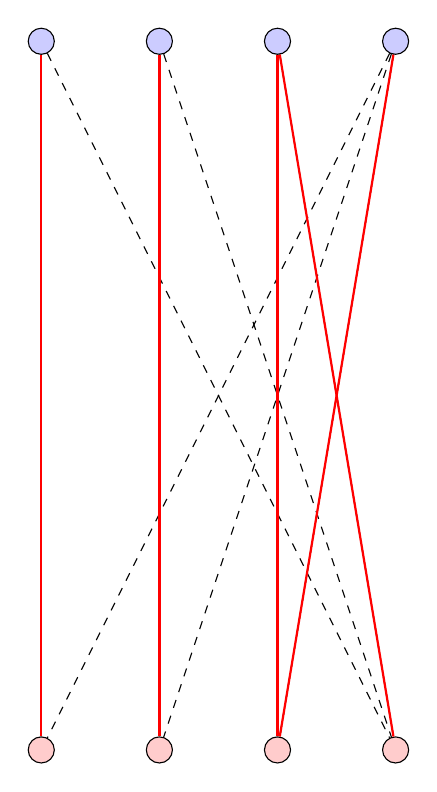
\begin{tikzpicture}[scale=1.5]
    % Define the vertices
    \foreach \i in {1,...,4} {
        \node[circle, draw, fill=blue!20] (A\i) at (\i,3) {};
        \node[circle, draw, fill=red!20] (B\i) at (\i,-3) {};
    }

    % Draw all edges except for the edge connecting A4 and B4
    \foreach \i in {1,...,3} {
        \draw[thick] (A\i) -- (B\i);
        \draw[dashed] (A\i) -- (B4);
        \draw[dashed] (A4) -- (B\i);
    }
    \draw[dashed] (A3) -- (B4);
    \draw[dashed] (A4) -- (B3);

    % Highlight the edges offered by Waiter in each round
    \foreach \i in {1,...,3} {
        \draw[thick, red] (A\i) -- (B\i);
        \pause % This command is used in Beamer to pause between rounds
    }
    \draw[thick, red] (A3) -- (B4);
    \draw[thick, red] (A4) -- (B3);

\end{tikzpicture}

\end{document}